\documentclass[11pt]{standalone}
\usepackage{tikz, pgfplots,amsmath, amssymb, amsthm}   
\usepgfplotslibrary{groupplots}


\begin{document}





\tikzset{every picture/.style={line width=0.75pt}} %set default line width to 0.75pt        

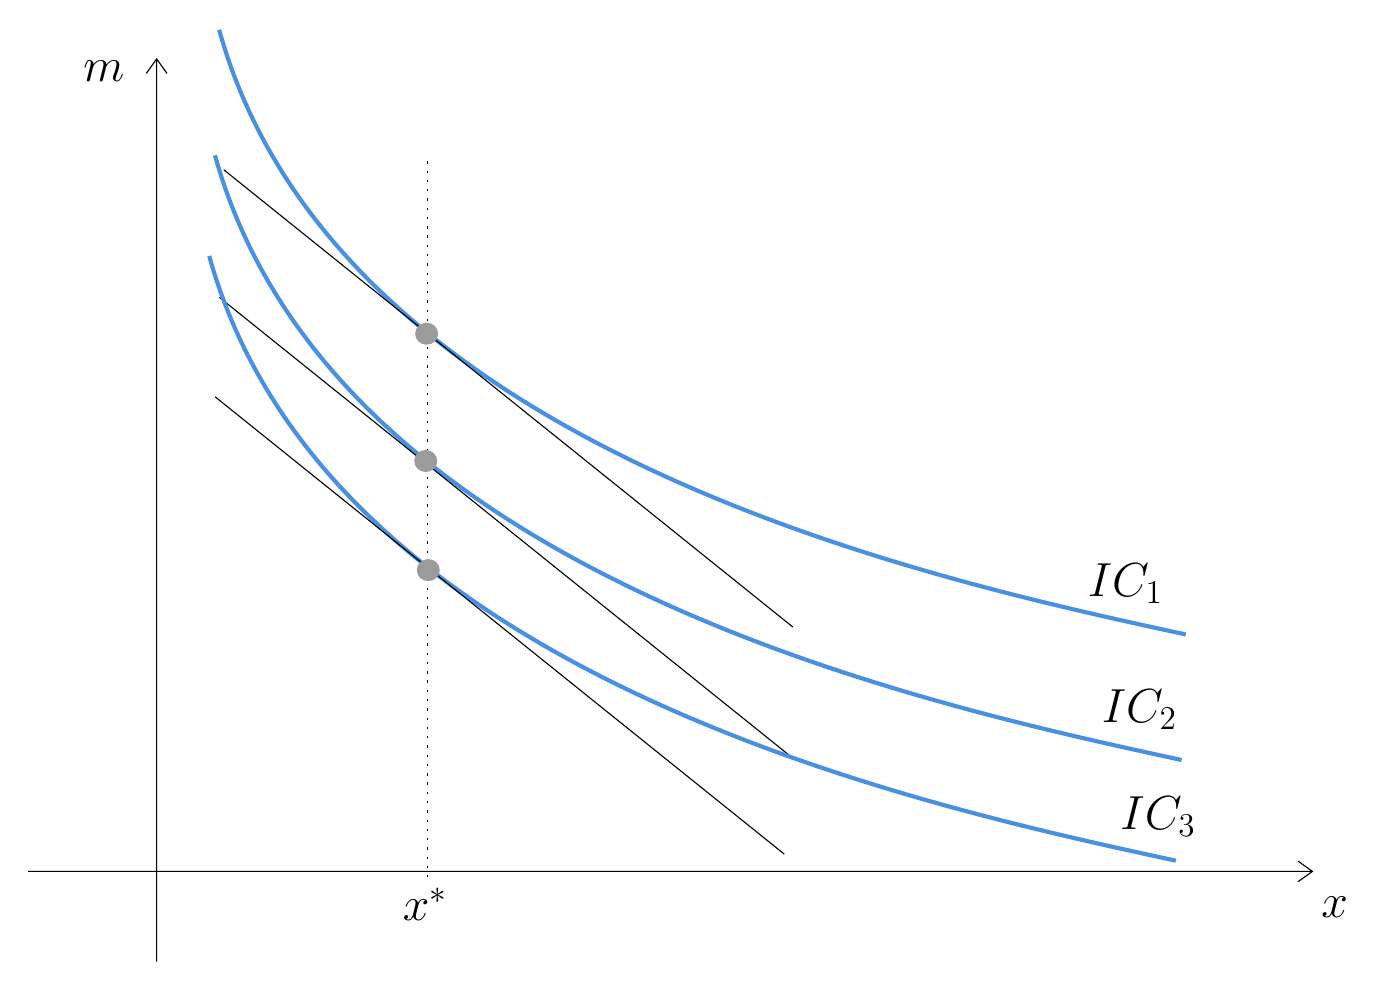
\begin{tikzpicture}[x=0.75pt,y=0.75pt,yscale=-1,xscale=1]
%uncomment if require: \path (0,466.0242919921875); %set diagram left start at 0, and has height of 466.0242919921875

%Shape: Axis 2D [id:dp9201480428116793] 
\draw  (4.5,437.54) -- (623.23,437.54)(66.37,46.08) -- (66.37,481.03) (616.23,432.54) -- (623.23,437.54) -- (616.23,442.54) (61.37,53.08) -- (66.37,46.08) -- (71.37,53.08)  ;
%Curve Lines [id:da7243503921849692] 
\draw [color={rgb, 255:red, 74; green, 144; blue, 226 }  ,draw opacity=1 ][line width=1.5]    (94.47,92.51) .. controls (151.05,296.9) and (440.49,357.78) .. (560.18,383.87) ;


%Straight Lines [id:da5613762331223611] 
\draw    (96.64,161.01) -- (370.85,381.34) ;


%Straight Lines [id:da4522188969819001] 
\draw  [dash pattern={on 0.84pt off 2.51pt}]  (196.75,95.41) -- (196.75,440.4) ;


%Curve Lines [id:da946453531361598] 
\draw [color={rgb, 255:red, 74; green, 144; blue, 226 }  ,draw opacity=1 ][line width=1.5]    (91.7,141.03) .. controls (148.28,345.41) and (437.72,406.29) .. (557.41,432.38) ;


%Straight Lines [id:da16858756761660243] 
\draw    (94.55,208.88) -- (368.76,429.2) ;


%Curve Lines [id:da8147789426111685] 
\draw [color={rgb, 255:red, 74; green, 144; blue, 226 }  ,draw opacity=1 ][line width=1.5]    (96.49,32.03) .. controls (153.07,236.42) and (442.51,297.3) .. (562.2,323.39) ;


%Straight Lines [id:da13614208559678342] 
\draw    (98.67,99.45) -- (372.87,319.78) ;


%Shape: Ellipse [id:dp8105961190312634] 
\draw  [draw opacity=0][fill={rgb, 255:red, 155; green, 155; blue, 155 }  ,fill opacity=1 ] (190.92,178.48) .. controls (190.92,175.55) and (193.4,173.17) .. (196.46,173.17) .. controls (199.52,173.17) and (202,175.55) .. (202,178.48) .. controls (202,181.42) and (199.52,183.79) .. (196.46,183.79) .. controls (193.4,183.79) and (190.92,181.42) .. (190.92,178.48) -- cycle ;
%Shape: Ellipse [id:dp09543007995953912] 
\draw  [draw opacity=0][fill={rgb, 255:red, 155; green, 155; blue, 155 }  ,fill opacity=1 ] (190.47,239.79) .. controls (190.47,236.86) and (192.95,234.48) .. (196.01,234.48) .. controls (199.07,234.48) and (201.55,236.86) .. (201.55,239.79) .. controls (201.55,242.72) and (199.07,245.1) .. (196.01,245.1) .. controls (192.95,245.1) and (190.47,242.72) .. (190.47,239.79) -- cycle ;
%Shape: Ellipse [id:dp4943064660201968] 
\draw  [draw opacity=0][fill={rgb, 255:red, 155; green, 155; blue, 155 }  ,fill opacity=1 ] (191.71,292.35) .. controls (191.71,289.42) and (194.19,287.04) .. (197.25,287.04) .. controls (200.31,287.04) and (202.79,289.42) .. (202.79,292.35) .. controls (202.79,295.29) and (200.31,297.66) .. (197.25,297.66) .. controls (194.19,297.66) and (191.71,295.29) .. (191.71,292.35) -- cycle ;


% Text Node
\draw (40.94,51.86) node   {\LARGE$m$};
% Text Node
\draw (633.96,454.59) node   {\LARGE$x$};
% Text Node
\draw (195.78,453.51) node   {\LARGE$x^{*}$};
% Text Node
\draw (533.18,299.03) node   {\LARGE$IC_{1}$};
% Text Node
\draw (539.94,359.47) node   {\LARGE$IC_{2}$};
% Text Node
\draw (548.95,411.28) node   {\LARGE$IC_{3}$};


\end{tikzpicture}



\end{document}